\scanpage{6}
\uline{UNIVERSITÀ DI PISA}

ISTITUTO MATEMATICO ``LEONIDA TONELLI''
\figure{\begin{tikzpicture}\draw (-1,0)--(-.1,0);\fill (-.08,-.025) rectangle (.08,.025);\draw (.1,0)--(1,0);\end{tikzpicture}}
\figure{
\begin{tikzpicture}[x=.01cm,y=-.01cm,line width=.4pt,draw=gray!25]
\foreach \x in {320,520,720} {
\draw (\x,0)--(\x,-90)--(\x+32,-90)--(\x+38,-65)--(\x+62,-43)--(\x+90,-43)--(\x+110,-18)--(\x+90,5)--(\x+62,5)--(\x+38,30)--(\x+32,55)--(\x,55)--cycle;
\draw (\x,-55)--(\x+32,-55) (\x,-38)--(\x+32,-38) (\x,15)--(\x+32,15) (\x+62,-43)--(\x+62,5) (\x+78,-43)--(\x+78,5) (\x+90,-33)--(\x+102,-18)--(\x+90,-3);
}
\draw (15,-35) to[out=-10,in=-170] (65,-37) to[out=160,in=-10] (10,-50)--(8,-15)--(20,-10)--(22,-30);
\draw (37,-30)--(36,-8)--(53,-10)--(54,-32);
\draw (96,-48) to[out=10,in=170] (150,-47) to[out=190,in=20] (95,-20)--(148,-10) to[out=160,in=-30] (106,-30)--(153,-43);
\draw (925,-30) to[out=-150,in=-130] (970,-35) to[out=-120,in=-30] (926,-24);
\draw (980,-25)--(991,-45)--(1000,-5)--(1020,-5)--(1013,-30)--(1000,-5);
\draw (1035,-30)--(1038,-2)--(1082,0)--(1085,-27) to[out=-170,in=-10] (1035,-30) to[out=10,in=170] (1085,-27);
\end{tikzpicture}}
\unsure{Arrive verci|Arrive derci}

\figure{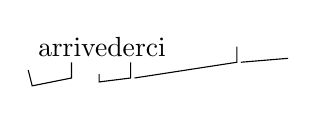
\begin{tikzpicture}[x=1cm,y=1cm]
\node[anchor=west] at (0,.4) {arrivederci};
\draw (0,.1)--(.05,-.1)--(.55,0)--(.55,.2);
\draw (.9,.05)--(.9,-.05)--(1.3,0)--(1.3,.2);
\draw (1.35,0)--(2.65,.2)--(2.65,.4);
\draw (2.7,.2)--(3.3,.25);
\end{tikzpicture}}
\[
\left[\begin{array}{l}
\text{buon giorno}\\
\text{\unsure{buona} sera}\\
\text{buona notte}\\
\text{per favore}\\
\text{mangare}\\
\text{\unsure{collazione|colazione}}
\end{array}\right.
\]
\figure{\begin{tikzpicture}[x=.01cm,y=-.01cm,line width=.7pt]
\node[rotate=90,anchor=west] at (90,-30) {Corso Italia};
\node[rotate=45,anchor=west] at (122,-140) {\unsure{Pizzeria}};
\draw (100,0)--(102,76)--(0,84);
\draw (155,0)--(158,73)--(370,72);
\draw (15,145)--(100,142);
\draw (165,132)--(320,132);
\draw (110,155)--(112,353)--(103,350);
\draw (160,162)--(158,340)--(340,346);
\draw (8,343)--(96,341);
\draw (0,400)--(95,398);
\draw (155,400)--(350,400)--(355,435)--(435,433)--(437,407)--(370,399);
\node at (398,415) {$\unsure{v}$};
\draw (112,400)--(120,510)--(126,504);
\draw (118,416)--(118,596);
\draw[->] (183,400)--(181,571);
\draw (215,460) .. controls (230,445) and (228,585) .. (210,600) .. controls (250,610) and (250,740) .. (212,768) .. controls (250,785) and (248,936) .. (214,946);
\draw (440,538)--(588,527);
\draw (435,540)--(440,660)--(570,660);
\draw (605,539)--(603,620)--(594,652);
\draw (608,641)--(613,663)--(585,666);
\end{tikzpicture}}
\mspage{5}
